%* 
%* ------------------------------------------------------------------
%* MainWindows.tex - General purpose Main Windows
%* Created by Robert Heller on Thu Apr 19 14:41:50 2007
%* ------------------------------------------------------------------
%* Modification History: $Log$
%* Modification History: Revision 1.2  2007/11/30 13:56:50  heller
%* Modification History: Novemeber 30, 2007 lockdown.
%* Modification History:
%* Modification History: Revision 1.1  2007/05/06 12:49:38  heller
%* Modification History: Lock down  for 2.1.8 release candidate 1
%* Modification History:
%* Modification History: Revision 1.1  2002/07/28 14:03:50  heller
%* Modification History: Add it copyright notice headers
%* Modification History:
%* ------------------------------------------------------------------
%* Contents:
%* ------------------------------------------------------------------
%*  
%*     Model RR System, Version 2
%*     Copyright (C) 1994,1995,2002-2005  Robert Heller D/B/A Deepwoods Software
%* 			51 Locke Hill Road
%* 			Wendell, MA 01379-9728
%* 
%*     This program is free software; you can redistribute it and/or modify
%*     it under the terms of the GNU General Public License as published by
%*     the Free Software Foundation; either version 2 of the License, or
%*     (at your option) any later version.
%* 
%*     This program is distributed in the hope that it will be useful,
%*     but WITHOUT ANY WARRANTY; without even the implied warranty of
%*     MERCHANTABILITY or FITNESS FOR A PARTICULAR PURPOSE.  See the
%*     GNU General Public License for more details.
%* 
%*     You should have received a copy of the GNU General Public License
%*     along with this program; if not, write to the Free Software
%*     Foundation, Inc., 675 Mass Ave, Cambridge, MA 02139, USA.
%* 
%*  
%* 

\chapter{Creating Main Windows}
\label{chapt:MainWindows}
\typeout{$Id$}

To aid in creating standardized main windows with some common
``trimmings'', the Model Railroad System includes a package that
enhances and extends the BWidget MainWindow widget.  The enhanced main
window widget is a Snit widgetadaptor that adds a BWidget
ScrolledWindow, an enhanced PanedWindow, a ButtonBox, and
``slideouts''\footnote{See Section~\ref{sec:Main:Slideouts} for more
information about slideouts.} to the body of the BWidget MainWindow. 
Along with the enhanced main window, there is also code available for a
standardized menu bar\footnote{See Section~\ref{sec:Main:StdMenuBar} for
more information about the standardized menu bar.}.

\section{What is in an enhanced Main Window?}
\label{sec:Main:WhatIsIn}

An enhanced Main Window is a BWidget MainWindow\index{Main
Windows!MainWindow, BWidget in}, with an enhanced PanedWindow\index{Main
Windows!PanedWindow (enhanced), BWidget in}, with a ScrolledWindow\index{Main
Windows!ScrolledWindow, BWidget in} on the left and a vertical
ButtonBox\index{Main Windows!ButtonBox, BWidget in} on the right, with zero
or more optional ``slideouts'' to the right of the vertical ButtonBox. 
The ScrolledWindow can contain any scrollable widget, such as a text
window (for log output), a canvas (for graphical output), a ListBox or
Tree widget, or a ScrolledFrame.  The vertical ButtonBox can be used
for a vertical collection of command buttons.

\subsection{Slideouts}
\label{sec:Main:Slideouts}

Slideouts are additional frames that can
be ``slid'' out (exposed to the right) as needed and then slid back in
(withdraw from view) when no longer needed.  Useful for GUI elements
that don't need to be displayed all of the time.  Any number of these
slideouts can be created and any subset of them can be displayed at any
time.

\subsection{Standard Menu Bars}
\label{sec:Main:StdMenuBar}

The BWStdMenuBar package
defines code for a standardized menu bar containing a File, Edit, View,
Options, and Help drop down menus.  The File, Edit, and Help menus are
populated with standard menu items.


\section{Creating a typical Main Window}
\label{sec:Main:SampleMainWindow}

\lstinputlisting[caption={Creating a Main Window},
		 label={lst:Main:MainWindowCode},
		 firstline=39]{SampleCodeMain.tcl}
\begin{figure}[hbpt]
\begin{centering}
\includegraphics[width=5in]{MainWindow1.png}
\caption{Sample Main Window, slideout hidden}
\label{fig:Main:MainWindow1}
\end{centering}
\end{figure}
\begin{figure}[hbpt]
\begin{centering}
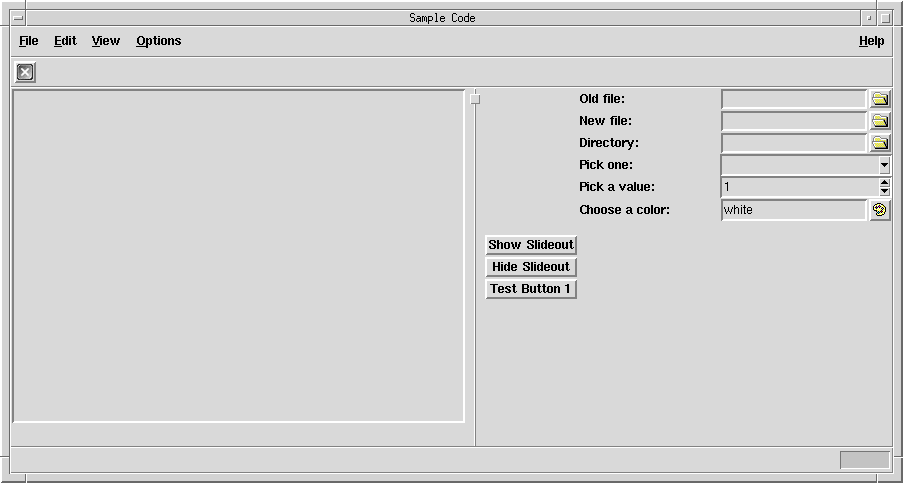
\includegraphics[width=5in]{MainWindow2.png}
\caption{Sample Main Window, slideout shown}
\label{fig:Main:MainWindow2}
\end{centering}
\end{figure}
Listing~\ref{lst:Main:MainWindowCode} contains code to create a basic
Main Window with a canvas window, simple set of command buttons, and a
slideout\footnote{See Chapter~\ref{chapt:LabelFrameWidgets} for the code used
to populate the slideout.}.  The window this code creates is shown in
Figures~\ref{fig:Main:MainWindow1} and \ref{fig:Main:MainWindow2}.
